
\documentclass{article}
\usepackage[utf8]{inputenc}

\title{Hammond_project}
\author{shahed_iasir }
\date{\today}

\usepackage{natbib}
\usepackage{graphicx}
\graphicspath{{images/}}
\usepackage{float}
\usepackage{setspace}

\usepackage{listings} % for writing the matlab code
%-----------for hyper reference------
\usepackage{hyperref}




\begin{document}

\noindent CH{\_}ENG 8452:\textsc{  Advanced Chemical Engineering Thermodynamics II} \\
\textsc{Assignment 5}\\
May 3, 2017 \\
To : Dr. \textsc{Karl Hammond} \\
From: \textsc{Abu Rafi Mohammad Iasir}\\
Mail: \href{mailto:ai9tb@mail.missouri.edu}{ai9tb@mail.missouri.edu}

%\maketitle
\begin{doublespacing}

\begin{figure}[H]
\begin{center}
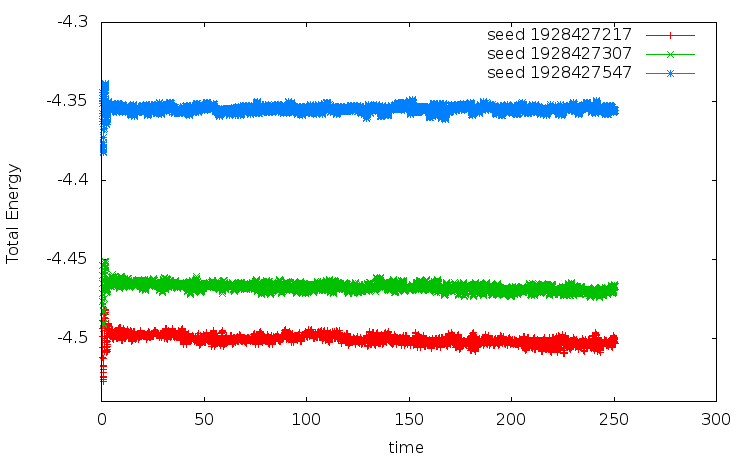
\includegraphics[scale=0.8]{Energy_vs_step} 
\caption{Energy vs time plot for LAMMPS simulation}  
\label{EV_lammps} 
\end{center}
\end{figure}
\begin{figure}[H]
\begin{center}
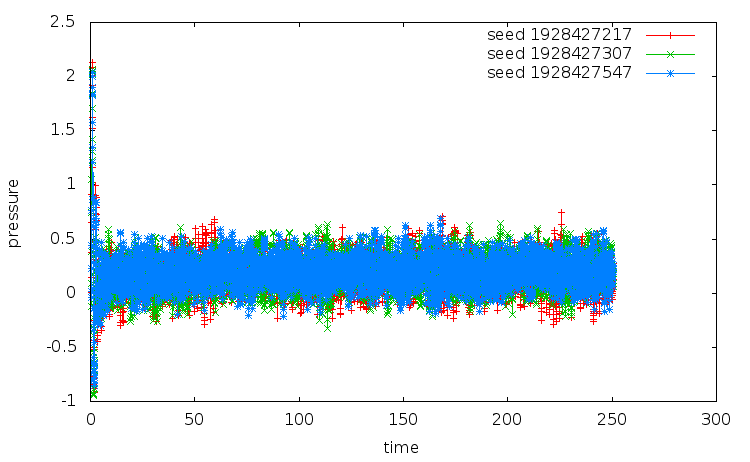
\includegraphics[scale=0.8]{pressure_vs_time} 
\caption{Pressure vs time plot for LAMMPS simulation}  
\label{PV_lammps} 
\end{center}
\end{figure}

\begin{figure}[H]
\begin{center}
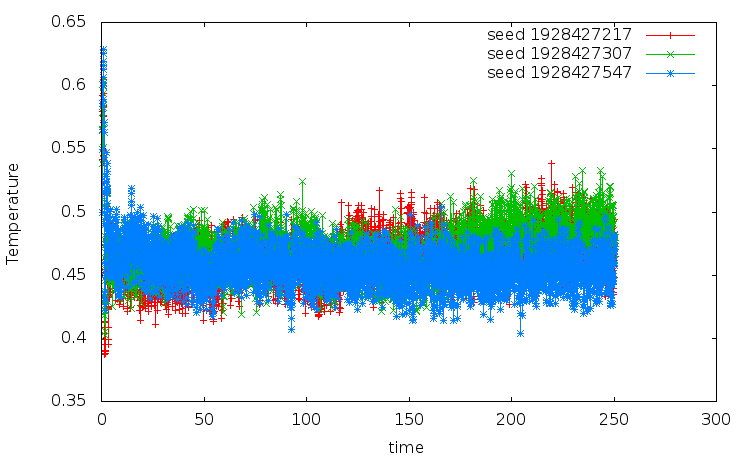
\includegraphics[scale=0.8]{temp_vs_time} 
\caption{Temperature vs time for LAMMPS simulation}  
\label{TV_lammp} 
\end{center}
\end{figure}

\begin{figure}[H]
\begin{center}
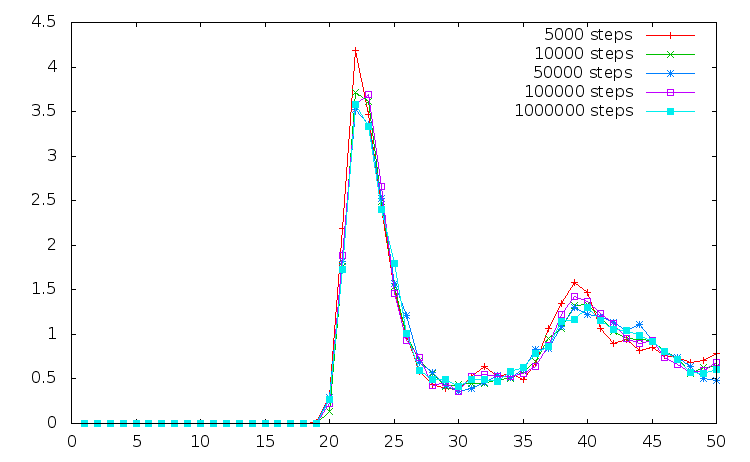
\includegraphics[scale=0.8]{RDF_MD} 
\caption{Radial distribution function plot from LAMMPS simulation}
\label{RDF_lammp} 
\end{center}
\end{figure}

\begin{figure}[H]
\begin{center}
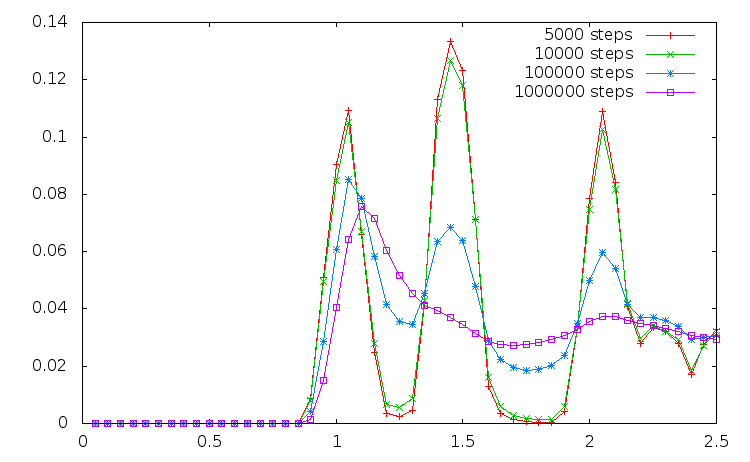
\includegraphics[scale=0.8]{RDF_MC} 
\caption{Radial distribution function plot from Monte Carlo program}
\label{RDF_MC}
\end{center}
\end{figure}

2. Figure \ref{EV_lammps} shows the change of energy with respect to time. Energy , temperature(\ref{PV_lammps}) and pressure (\ref{TV_lammps}) plots are included in the report. Actual thermodynamic propertis (i.e energy, temperature and pressure) should be the average value of the data. Since MD simulation mainly deals with microcanonical ensemble.

\section{Conclusion}


\end{doublespacing}


\bibliographystyle{plain}
\newpage
\bibliography{references}

\end{document}
